\chapter{Sounds of the General American English}
\label{chap:english_language}
In the \textit{General American English} there are 41 different sounds in which can be structured by the way they are produced. In \ref{table:english_sounds} is shown the kind of sounds with the respective number of possible productions. Each type will be described into a dedicated section of this thesis. An important factor is the way of how the \textit{constriction} of the flow of air is made. In fact, to distiguish between \textit{consonants}, \textit{semivowels} and \textit{vowels}, the \textit{degree} of constriction is checked. Instead, for \textit{sonorant} consonants the air flow is continuous with no pressure. \textit{Nasal} consonants have an occlusive consonant made with a lowered velum allowing the airflow in the nasal cavity \cite{nasal_cons_wiki}. The \textit{continuant} consonants are produced without blocking the airflow in the oral cavity.

\begin{table}[h]
    \centering
    \begin{tabular}{|c|c|}
        \hline
        \textbf{Type}& \textbf{Number} \\ \hline
        Vowels     & 18     \\ \hline
        Fricatives & 8      \\ \hline
        Stops      & 6      \\ \hline
        Nasals     & 3      \\ \hline
        Semivowels & 4      \\ \hline
        Affricates & 2      \\ \hline
        Aspirant   & 1      \\ \hline
    \end{tabular}
    \caption {Type of English sounds}
\label{table:english_sounds}
\end{table}

\section{Vowel production}
\label{sec:vowel_production}
Generally speaking, when a vowel is pronunced, there is no air-constriction in the flow. This means that the ariculators like the tongue, lips and the uvula do not touch allowing the flow of air from the lungs. The consonants instead have another pattern when producing them. Moreover, to produce each vowel, the mouth has to make a different shape in such a way that the resonance is different. \ref{fig:vowels_prod} shows the way the mouth, the jaw and the lips are combined in a such a way to produce the acoustinc sound of a vowel.

\begin{figure}[!ht]
    \centering
    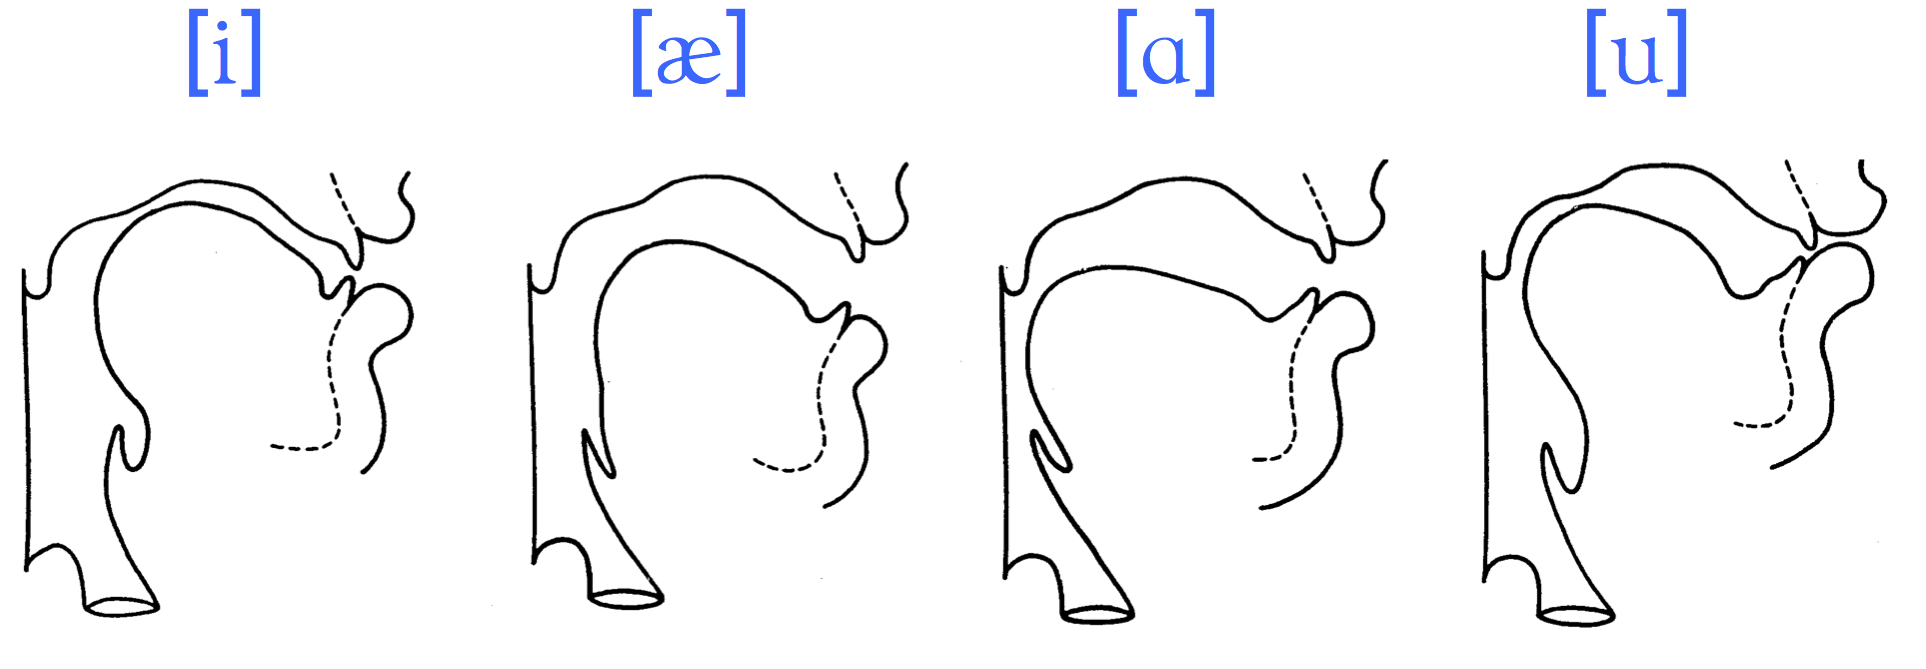
\includegraphics[scale=0.5]{Figures/vowels_prod.png}
    \caption{Vowels production} % \cite{mit_phonetics} RICORDATI DI INSERIRE QUESTA CITAZIONE PRIMA DI PUBBLICARE
    \label{fig:vowels_prod}
\end{figure}

\subsection{Vowel of American English}
\label{sub:vowel_of_american_english}
There are 18 different vowels in American English that can be grouped by three different sets: the \textbf{monopthongs}, the \textbf{diphthongs}, and the \textbf{schwa's} - or reduced vowels.

\begin{figure}[!ht]
    \centering
    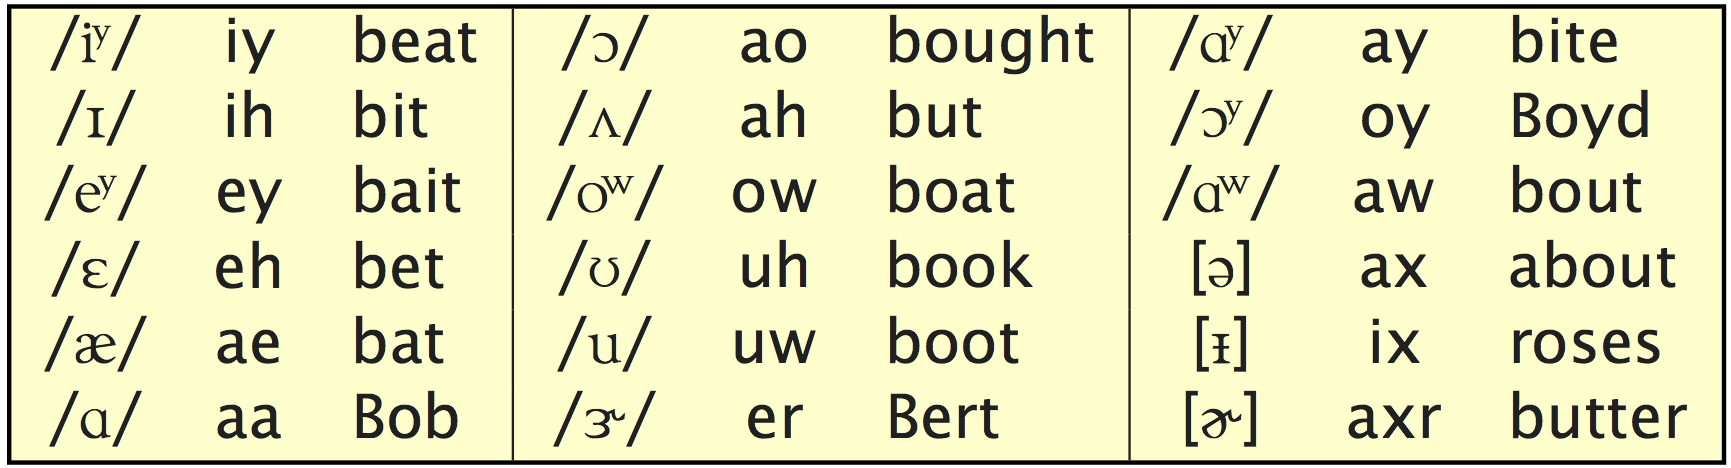
\includegraphics[scale=0.5]{Figures/vowels_sets.png}
    \caption{Example of words depending on the group} % \cite{mit_phonetics} RICORDATI DI INSERIRE QUESTA CITAZIONE PRIMA DI PUBBLICARE
    \label{fig:vowels_prod}
\end{figure}

The first column shows some examples of monopthongs. A \textit{monopthong} is a clear vowel sound in which the utterance are fixed at both the beginning and at the end. The central part of the picture represents the dipthongs. A \textit{dipthong} is the sound produced by two vowels when they occur within the same syllable \cite{dipthong_wiki}. In the last column are depictes some examples of reduced vowels. \textit{Schwa's} refers to the vowel sound that stays in the mid-central of the word. In general, in the english language, the schwa is found in unstressed position \cite{schwa_wiki}.

\subsection{Formants}
\label{sub:formants}
A \textit{formant} is the resonant frequency of a vocal track that resonate the loudest. In a spectrum graph, formants are represented by the peaks. In \ref{fig:peaks_formants} it is possibile to see how the three first formants are defined by the peaks. The pictures is the \textit{envelope} of a spectogram of the vowel \textbf{[i]}. Frequencies are the most relevant information to determine which vowel has been pronounced. In general, within a spectrum graph there may be a different number of formants, although the most relevant are the first three and they are named \textbf{F1}, \textbf{F2} and \textbf{F3}.

\begin{figure}[!ht]
    \centering
    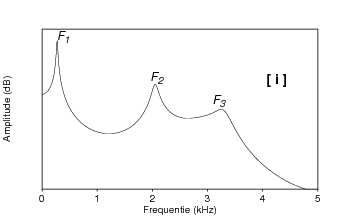
\includegraphics[scale=0.5]{Figures/peaks_formants.png}
    \caption{Spectral envelope of the [i] vowel pronunciation. F1, F2 and F3 are the first 3 formants \cite{formants_peaks}}
    \label{fig:peaks_formants}
\end{figure}

\subsection{Vowel Formant Averages}
\label{sub:vowel_formant_averages}

\subsection{Vowel duration}
\label{sub:vowel_duration}


\section{Fricative Production}
\label{sec:fricative_production}


\subsection{Fricatives of American English}
\label{sub:Fricatives of American English}


\subsection{Fricative Energy and Duration}
\label{sub:Fricative Energy and Duration}


\section{Stop Production}
\label{sec:Stop Producton}


\subsection{Stops of American English}
\label{sub:Stops of American English}


\section{Nasal Production}
\label{sec:Nasal Production}


\subsubsection{Nasal of American English}
\label{subs:Nasal of American English}


\section{Semivowels Production}
\label{sec:Semivowels Production}


\subsection{Semivowels of American English}
\label{sub:Semivowels of American English}


\subsection{Acousitc Properties of Semivowels}
\label{sub:Acousitc Properties of Semivowels}

\section{Affricate Production}
\label{sec:Affricate Production}


\section{Aspirant Production}
\label{sec:Aspirant Production}


\section{Phonotactic Constraints}
\label{sec:Phonotactic Constraints}


\section{The Syllable}
\label{sec:The syllable}


\subsection{Syllables and Sonority}
\label{sub:Syllables and Sonority}
